\section{Fabricación de alimentos}
\subsection{Enunciado 12-1} 
\paragraph{}Un alimento se fabrica refinando aceites crudos y mezclandolos. Los aceites crudos son de dos categorias:
\begin{center}
\begin{tabular}{@{}cl@{}}
\hline
\multirow{2}{*}{\begin{tabular}[c]{@{}c@{}}Aceites vegetales\end{tabular}}     & Veg 1 \\
                                                                                  & Veg 2 \\
\multirow{3}{*}{\begin{tabular}[c]{@{}c@{}}Aceites no vegetabes\end{tabular}} & Oil 1 \\
                                                                                  & Oil 2 \\
                                                                                 & Oil 3\\
                                                                                 \hline 
\end{tabular}
\end{center}
\paragraph{}Cada aceite puede comprarse para entrega inmediata (enero) o comprarse en el mercado para una entrega futura en un mes posterior. Los precios se indican a continuacion(\pounds /ton):\\

\begin{center}
\begin{tabular}{|c|c|c|c|c|c|}
\hline 
 & Veg 1 & Veg 2 & Oil 1 & Oil 2 & Oil 3 \\ 
\hline 
Enero & 110 & 120 & 130 & 110 & 115 \\ 
\hline 
Febrero & 130 & 130 & 110 & 90 & 115 \\ 
\hline 
Marzo & 110 & 140 & 130 & 100 & 95 \\ 
\hline 
Abril & 120 & 110 & 120 & 120 & 125 \\ 
\hline 
Mayo & 100 & 120 & 150 & 110 & 105 \\ 
\hline 
Junio & 90 & 100 & 140 & 80 & 135 \\ 
\hline 
\end{tabular} 
\end{center}

\paragraph{}El producto final se vende a \pounds 150 por tonelada.
\paragraph{}Los aceites vegetales y los aceites no vegetales requieren diferentes lineas de producción para refinar. En cualquier mes, no es posible refinar mas de 200 toneladas de aceites vegetales y mas de 250 toneladas de aceites no vegetales. No hay perdida de peso en el proceso de refinación y el costo de refinacion puede ser ignorado.
\paragraph{}Es posible almacenar hasta 1000 toneladas de cada aceite crudo para su uso posterior. El costo de almacenamiento para el aceite vegetal y no vegetal es de \pounds 25 por tonelada por mes. El producto final no se puede almacenar, ni se pueden almacenar aceites refinados.
\paragraph{}Hay una restricción tecnologica de dureza en el producto final. En las unidades de las que se mide la dureza, esta debe estar entre 3 y 6. Se supone que la dureza se combina linealmente y que las durezas de los aceites crudos son:\\
\begin{center}
\begin{tabular}{|c|c|}
\hline 
Veg 1 & 8.8 \\ 
\hline 
Veg 2 & 6.1 \\ 
\hline 
Oil 1 & 2.0 \\ 
\hline 
Oil 2 & 4.2 \\ 
\hline 
Oil 3 & 5.0 \\ 
\hline 
\end{tabular} 
\end{center}

\paragraph{}¿Que políticas de compras y fabricación debería seguir la empresa para maximizar los beneficios?  
\paragraph{}En la actualidad hay 500 toneladas de cada tipo de aceite crudo almacenado. Se requiere que estas existencias también existan a fines de junio.

\subsection{Modelo}
$\begin{array}{l}
Cv_{i,j}: \mbox{cantidad de toneladas de aceite vegetal crudo VEG i comprado en el mes j}\\
Co_{t,j}: \mbox{cantidad de toneladas de aceite no vegetal crudo OIL t comprado en el mes j}\\
Rv_{i,j}: \mbox{cantidad de toneladas de aceite vegetal crudo VEG i refinado en el mes j}\\
Ro_{t,j}: \mbox{cantidad de toneladas de aceite no vegetal crudo IOL t refinado en el mes j}\\
Av_{i,j}: \mbox{cantidad de toneladas de aceite vegetal crudo VEG i almacenado en el mes j}\\
Ao_{t,j}: \mbox{cantidad de toneladas de aceite no vegetal crudo IOL t almacenado en el mes j}\\
i=1,2  \;\;\;\;\;\; t=1,2,3 \;\;\;\;\;\; j=1,2,3,4,5,6\\ \\
\mbox{donde j representa los meses }1 \mbox{ es enero}, 2 \mbox{ es febrero, y asi.}
\end{array} $
\\ \\ 
$$\ \mbox{maxizar   } 150\left( \sum_{j=1}^{6}Rv_{1,j}+Rv_{2,j}+Ro_{1,j}+Ro_{2,j}+Ro_{3,j}\right) $$
$$\ - 25\left( \sum_{j=1}^{6}Av_{1,j}+Av_{2,j}+Ao_{1,j}+Ao_{2,j}+Ao_{3,j}\right) $$
$$\ - \left( 110Cv_{1,1}+130Cv_{1,2}+110Cv_{1,3}+120Cv_{1,4}+100Cv_{1,5}+90Cv_{1,6}\right) $$
$$\ - \left( 120Cv_{2,1}+130Cv_{2,2}+140Cv_{2,3}+110Cv_{2,4}+120Cv_{2,5}+100Cv_{2,6}\right) $$
$$\ - \left( 130Co_{1,1}+110Co_{1,2}+130Co_{1,3}+120Co_{1,4}+150Co_{1,5}+140Co_{1,6}\right) $$
$$\ - \left( 110Co_{2,1}+90Co_{2,2}+100Co_{1,3}+120Co_{1,4}+110Co_{1,5}+80Co_{1,6}\right) $$
$$\ - \left( 115Co_{3,1}+115Co_{3,2}+95Co_{1,3}+125Co_{1,4}+105Co_{1,5}+135Co_{1,6}\right) $$
\\ \\ 
s.a\\
No se pude refinar mas de 200 toneladas de aceite vegetales
\begin{equation}
Rv_{1,j} + Rv_{2,j} \leq 200 
\end{equation}
No se pude refinar mas de 250 toneladas de aceite no vegetales
\begin{equation}
Ro_{1,j} + Ro_{2,j} + Ro_{3,j} \leq 250 
\end{equation}
No se puede almacenar mas de 1000 toneledas de aceite vegetal
\begin{equation}
Av_{i,j} \leq 1000
\end{equation}
No se puede almacenar mas de 1000 toneledas de aceite no vegetal
\begin{equation}
Ao_{t,j} \leq 1000
\end{equation}
La dureza en el producto final debe ser mayor que 3 y menor que 6
\begin{equation}
 \frac{ 8.8 Rv_{1,j} + 6.1 Rv_{2,j} + 2.0 Ro_{1,j} + 4.2 Ro_{2,j} + 5.0 Ro_{3,j} } { Rv_{1,j} + Rv_{2,j} + Ro_{1,j} + Ro_{2,j} + Ro_{3,j}} \geq 3
\end{equation}
\begin{equation}
 \frac{8.8 Rv_{1,j} + 6.1 Rv_{2,j} + 2.0 Ro_{1,j} + 4.2 Ro_{2,j} + 5.0 Ro_{3,j}}{Rv_{1,j} + Rv_{2,j} + Ro_{1,j} + Ro_{2,j} + Ro_{3,j}} \leq 6
\end{equation}
Lo comprado + lo almacenado - lo refinado en el mes j, es lo almacenado para el mes j+1, para j=1,2,3,4,5
\begin{equation}
Cv_{i,j} + Av_{i,j} - Rv_{i,j} = Av_{i,j+1}
\end{equation}
\begin{equation}
Co_{t,j} + Ao_{t,j} - Ro_{t,j} = Ao_{t,j} 
\end{equation}
Lo comprado + lo almacenado - lo refinado en el mes de junio, es lo almacenado despues de junio
\begin{equation}
Cv_{i,6} + Av_{i,6} - Rv_{i,6} = Av_{i,7}
\end{equation}
\begin{equation}
Co_{t,6} + Ao_{t,6} - Ro_{t,6} = Ao_{t,7} 
\end{equation}
En enero se comienza con 500 toneladas de cada aceite almacenado y se quiere terminar junio con la misma cantidad
\begin{equation}
Av_{1,1}=500
\end{equation}
\begin{equation}
Av_{2,1}=500
\end{equation}
\begin{equation}
Ao_{1,1}=500
\end{equation}
\begin{equation}
Ao_{2,1}=500
\end{equation}
\begin{equation}
Ao_{3,1}=500
\end{equation}
\begin{equation}
Av_{1,7}=500
\end{equation}
\begin{equation}
Av_{2,7}=500
\end{equation}
\begin{equation}
Ao_{1,7}=500
\end{equation}
\begin{equation}
Ao_{2,7}=500
\end{equation}
\begin{equation}
Ao_{3,7}=500
\end{equation}

\subsection{Modelo CPLEX}
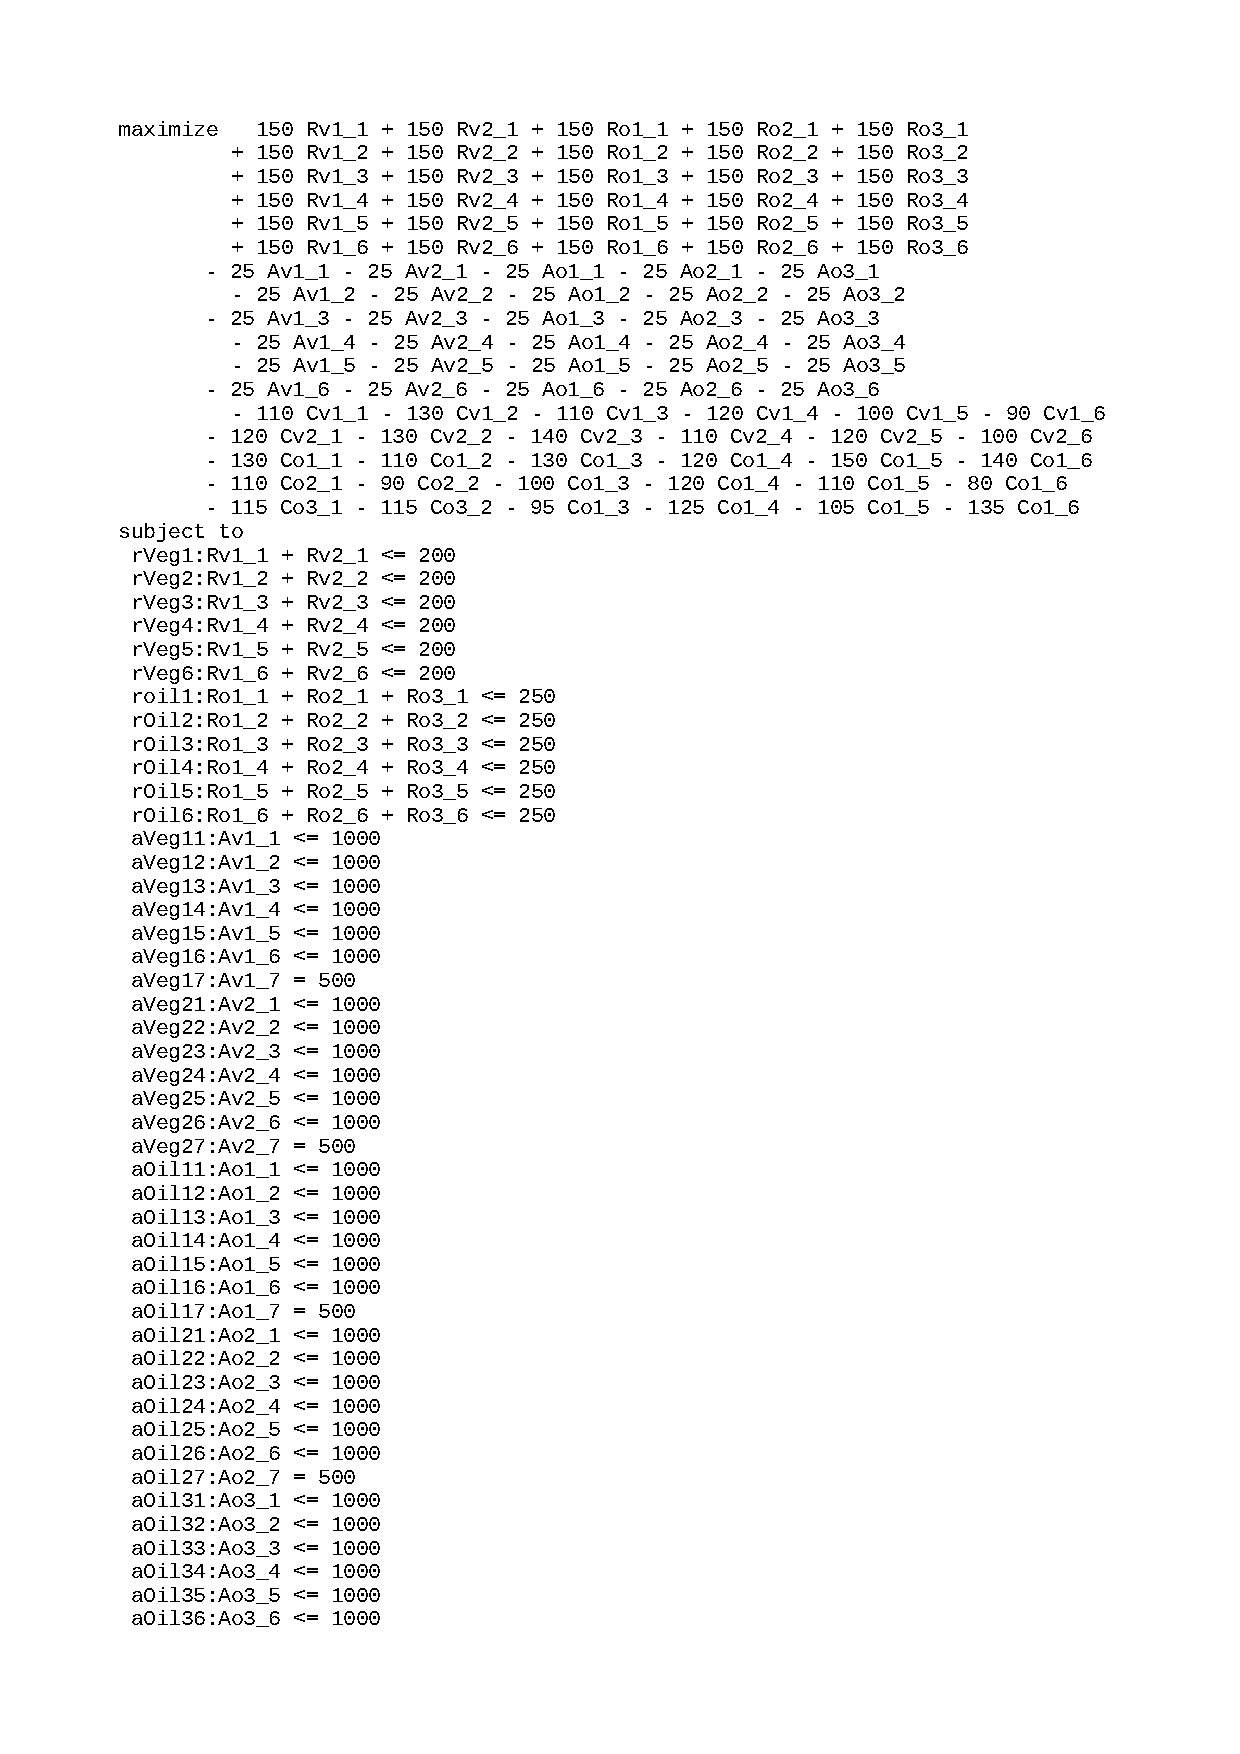
\includepdf[pages=1-2]{modelos/fabricaAlimentos12-1}


\subsection{Solucion CPLEX}
\paragraph{}¿Que políticas de compras y fabricación debería seguir la empresa para maximizar los beneficios?  

\begin{figure}[!h]
    \centering
    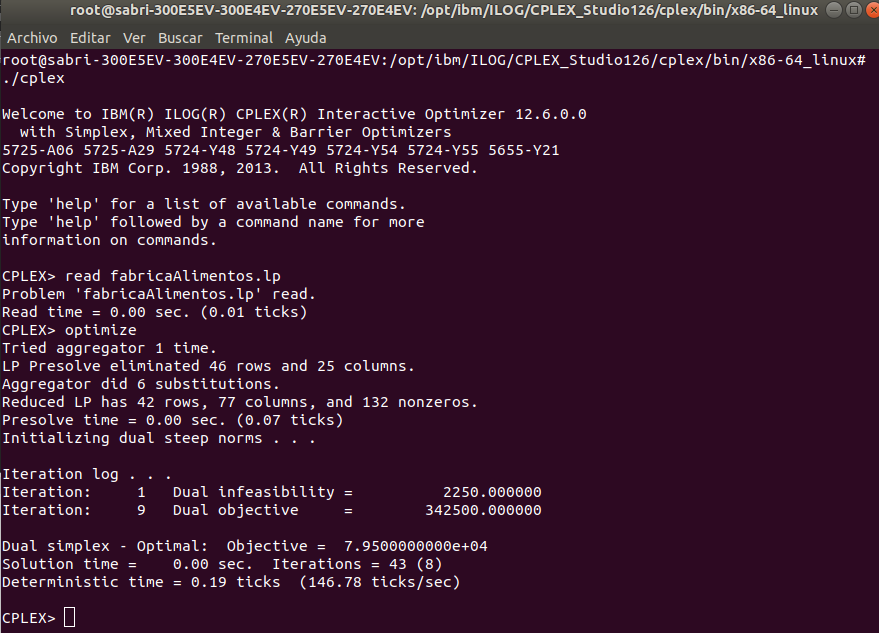
\includegraphics[scale=0.35]{modelos/fabricaAlimentos12-1Solucion.png}
    \caption{Solución}
\end{figure}

\begin{figure}[!h]
    \centering
    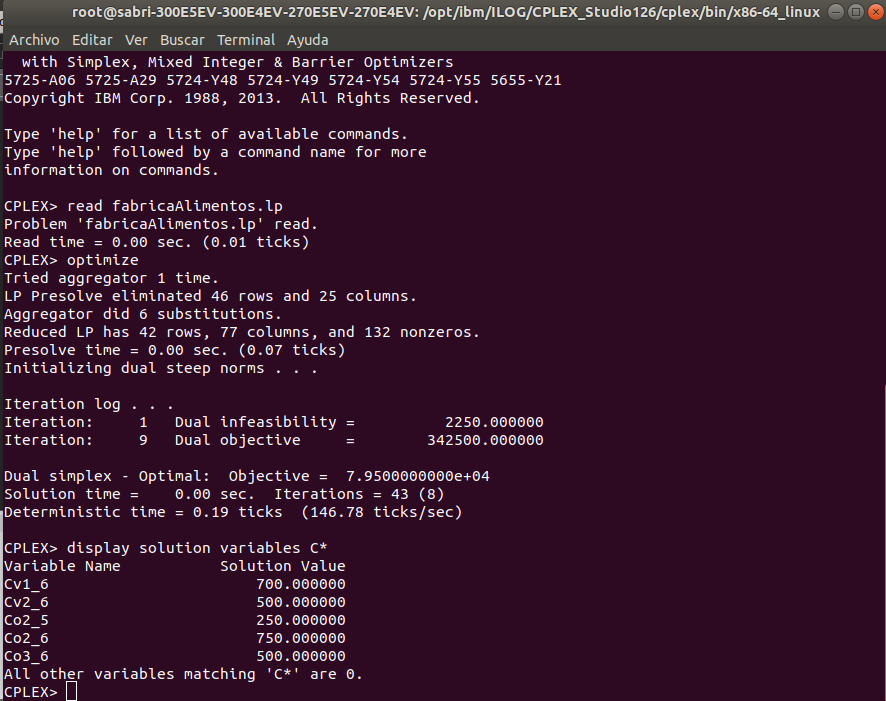
\includegraphics[scale=0.35]{modelos/fabricaAlimentos12-1Compras.png}
    \caption{Politicas de compras}
\end{figure}

\begin{figure}[!h]
    \centering
    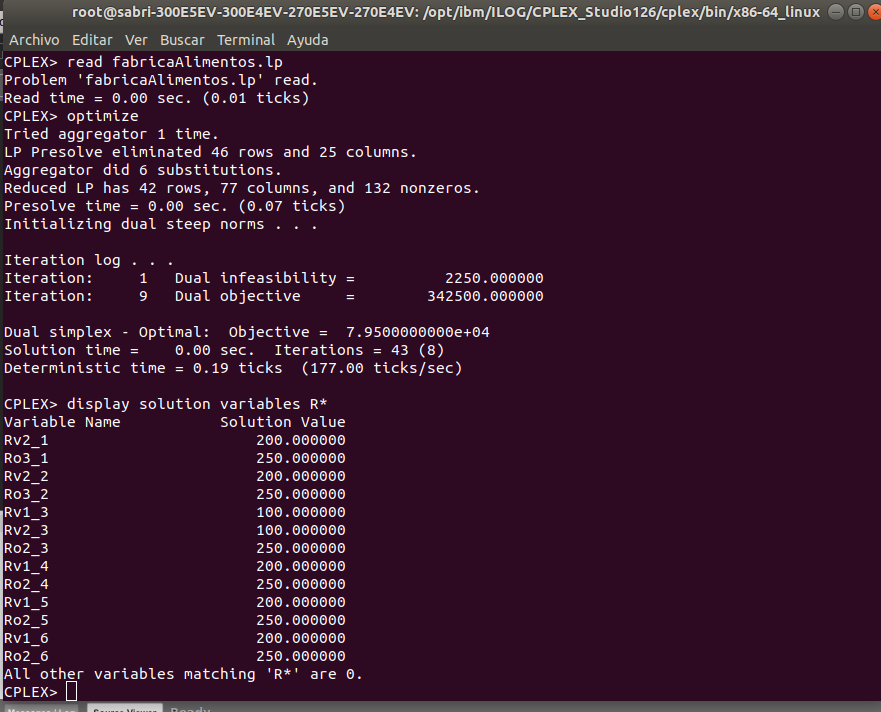
\includegraphics[scale=0.35]{modelos/fabricaAlimentos12-1Fabricacion.png}
    \caption{Politicas de fabricacion}
\end{figure}


\section{Fabricación de alimentos extensión}
\subsection{Enunciado 12-2}
\paragraph{}El problema y el problema posterior se basan en un modelo mas grande construido para el productor de margarina.
\paragraph{}Se desea imponer las siguientes condiciones adicionales al problema de la fabricación de alimentos.
\begin{itemize}
\item La comida nunca puede estar compuesta de mas de tres aceites en un mes.
\item Si se usa un aceite en un mes, se deben usar al menos 20 toneladas.
\item Si se utiliza Veg 1 o Veg 2 en un mes, también se deben utilizar oil 3.
\end{itemize}
\subsection{Modelo 12-2}
$\begin{array}{l}
Xv_{i,j} = \left\{
\begin{array}{l l}
 1 & \mbox{si } Rv_{i,j}>0\\
 0 & sino
\end{array}
\right.\\
Xo_{t,j} = \left\{
\begin{array}{l l}
 1 & \mbox{si } Ro_{i,j}>0\\
 0 & sino
\end{array}
\right.
\end{array}$
\\ \\ 
s.a\\
\begin{equation}
Xv_{1,j} + Xv_{2,j} + Xo_{1,j} + Xo_{2,j} + Xo_{3,j} \leq 3
\end{equation}
\begin{equation}
Rv_{i,j} \geq 20 \times Xv_{i,j}
\end{equation}
\begin{equation}
Ro_{t,j} \geq 20 \times Xo_{t,j}
\end{equation}
\begin{equation}
Rv_{1,j} \leq Ro_{3,j}
\end{equation}
\begin{equation}
Rv_{2,j} \leq Ro_{3,j}
\end{equation}
